\begin{center}
\begin{adjustbox}{width=7cm, height=12cm, keepaspectratio}
\tikzset{every picture/.style={line width=0.75pt}} %set default line width to 0.75pt        

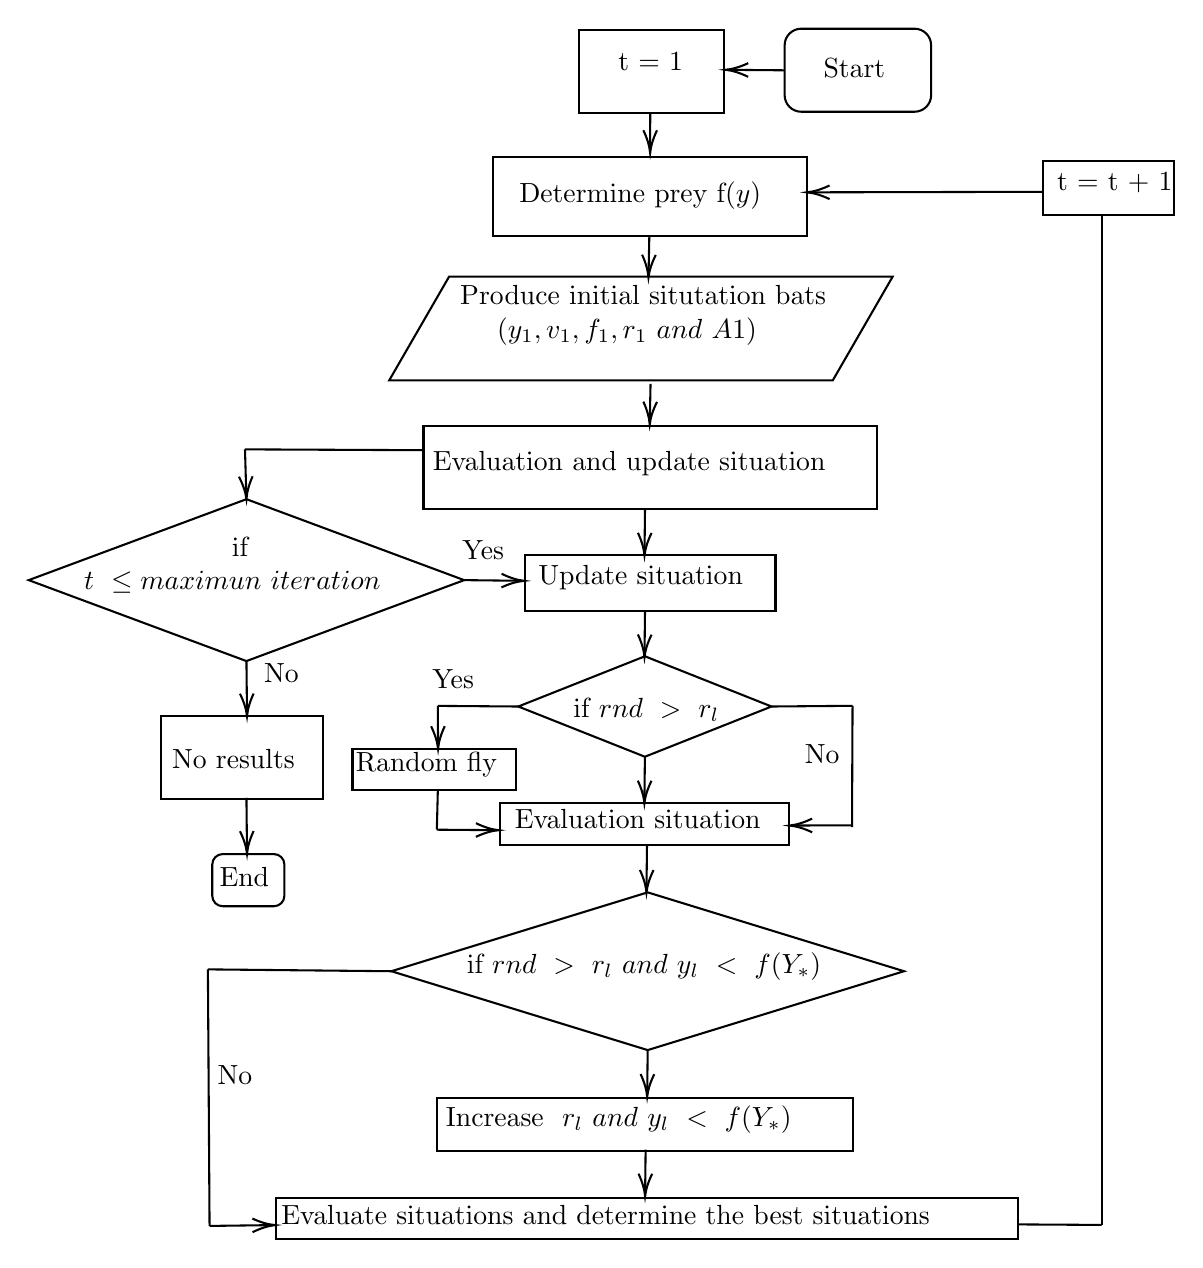
\begin{tikzpicture}[x=0.75pt,y=0.75pt,yscale=-1,xscale=1]
	%uncomment if require: \path (0,1122); %set diagram left start at 0, and has height of 1122
	
	%Shape: Rectangle [id:dp11199231081600236] 
	\draw   (288.02,34.47) -- (358.02,34.47) -- (358.02,74.47) -- (288.02,74.47) -- cycle ;
	
	%Shape: Rectangle [id:dp9862949515841928] 
	\draw   (246.6,95.5) -- (397.93,95.5) -- (397.93,133.67) -- (246.6,133.67) -- cycle ;
	
	%Rounded Rect [id:dp8968724601667921] 
	\draw   (387.27,41.8) .. controls (387.27,37.38) and (390.85,33.8) .. (395.27,33.8) -- (449.85,33.8) .. controls (454.27,33.8) and (457.85,37.38) .. (457.85,41.8) -- (457.85,65.8) .. controls (457.85,70.22) and (454.27,73.8) .. (449.85,73.8) -- (395.27,73.8) .. controls (390.85,73.8) and (387.27,70.22) .. (387.27,65.8) -- cycle ;
	
	%Straight Lines [id:da1448631814999326] 
	\draw    (387.02,53.84) -- (360.77,53.61) ;
	\draw [shift={(358.77,53.59)}, rotate = 0.51] [color={rgb, 255:red, 0; green, 0; blue, 0 }  ][line width=0.75]    (10.93,-3.29) .. controls (6.95,-1.4) and (3.31,-0.3) .. (0,0) .. controls (3.31,0.3) and (6.95,1.4) .. (10.93,3.29)   ;
	%Straight Lines [id:da08995180587744223] 
	\draw    (322.52,74.09) -- (322.47,91.67) ;
	\draw [shift={(322.47,93.67)}, rotate = 270.15] [color={rgb, 255:red, 0; green, 0; blue, 0 }  ][line width=0.75]    (10.93,-3.29) .. controls (6.95,-1.4) and (3.31,-0.3) .. (0,0) .. controls (3.31,0.3) and (6.95,1.4) .. (10.93,3.29)   ;
	%Shape: Rectangle [id:dp11994357769035191] 
	\draw   (225.6,153.27) -- (439.31,153.27) -- (410.44,203.27) -- (196.73,203.27) -- cycle ;
	
	%Shape: Rectangle [id:dp6991932005539763] 
	\draw   (213.27,225.07) -- (431.67,225.07) -- (431.67,265.07) -- (213.27,265.07) -- cycle ;
	
	%Straight Lines [id:da5570849935229241] 
	\draw    (322.07,134.07) -- (321.71,151.67) ;
	\draw [shift={(321.67,153.67)}, rotate = 271.17] [color={rgb, 255:red, 0; green, 0; blue, 0 }  ][line width=0.75]    (10.93,-3.29) .. controls (6.95,-1.4) and (3.31,-0.3) .. (0,0) .. controls (3.31,0.3) and (6.95,1.4) .. (10.93,3.29)   ;
	%Straight Lines [id:da23972455000161563] 
	\draw    (322.67,204.87) -- (322.31,222.47) ;
	\draw [shift={(322.27,224.47)}, rotate = 271.17] [color={rgb, 255:red, 0; green, 0; blue, 0 }  ][line width=0.75]    (10.93,-3.29) .. controls (6.95,-1.4) and (3.31,-0.3) .. (0,0) .. controls (3.31,0.3) and (6.95,1.4) .. (10.93,3.29)   ;
	
	%Shape: Rectangle [id:dp3372630993033694] 
	\draw   (262.07,287.27) -- (382.87,287.27) -- (382.87,314.21) -- (262.07,314.21) -- cycle ;
	
	%Shape: Diamond [id:dp22966171081387388] 
	\draw   (127.97,260.47) -- (232.87,299.47) -- (127.97,338.47) -- (23.07,299.47) -- cycle ;
	
	%Straight Lines [id:da2896807914403723] 
	\draw    (127.27,236.47) -- (213.27,236.87) ;
	%Straight Lines [id:da15189665526347684] 
	\draw    (127.27,236.47) -- (127.91,258.47) ;
	\draw [shift={(127.97,260.47)}, rotate = 268.33] [color={rgb, 255:red, 0; green, 0; blue, 0 }  ][line width=0.75]    (10.93,-3.29) .. controls (6.95,-1.4) and (3.31,-0.3) .. (0,0) .. controls (3.31,0.3) and (6.95,1.4) .. (10.93,3.29)   ;
	%Shape: Rectangle [id:dp751137217740556] 
	\draw   (87,364.88) -- (165,364.88) -- (165,404.88) -- (87,404.88) -- cycle ;
	%Straight Lines [id:da5722635336416755] 
	\draw    (127.97,338.07) -- (128.23,363.08) ;
	\draw [shift={(128.25,365.08)}, rotate = 269.4] [color={rgb, 255:red, 0; green, 0; blue, 0 }  ][line width=0.75]    (10.93,-3.29) .. controls (6.95,-1.4) and (3.31,-0.3) .. (0,0) .. controls (3.31,0.3) and (6.95,1.4) .. (10.93,3.29)   ;
	%Rounded Rect [id:dp3776201245469004] 
	\draw   (111.5,436.48) .. controls (111.5,433.71) and (113.75,431.46) .. (116.52,431.46) -- (141.22,431.46) .. controls (144,431.46) and (146.25,433.71) .. (146.25,436.48) -- (146.25,451.56) .. controls (146.25,454.33) and (144,456.58) .. (141.22,456.58) -- (116.52,456.58) .. controls (113.75,456.58) and (111.5,454.33) .. (111.5,451.56) -- cycle ;
	%Straight Lines [id:da8638079389758646] 
	\draw    (127.97,404.32) -- (128.23,429.33) ;
	\draw [shift={(128.25,431.33)}, rotate = 269.4] [color={rgb, 255:red, 0; green, 0; blue, 0 }  ][line width=0.75]    (10.93,-3.29) .. controls (6.95,-1.4) and (3.31,-0.3) .. (0,0) .. controls (3.31,0.3) and (6.95,1.4) .. (10.93,3.29)   ;
	%Straight Lines [id:da11071951771999644] 
	\draw    (232.87,299.47) -- (259.8,299.78) ;
	\draw [shift={(261.8,299.81)}, rotate = 180.67] [color={rgb, 255:red, 0; green, 0; blue, 0 }  ][line width=0.75]    (10.93,-3.29) .. controls (6.95,-1.4) and (3.31,-0.3) .. (0,0) .. controls (3.31,0.3) and (6.95,1.4) .. (10.93,3.29)   ;
	%Shape: Rectangle [id:dp7677856775494443] 
	\draw   (511.75,97.75) -- (574.74,97.75) -- (574.74,123.38) -- (511.75,123.38) -- cycle ;
	
	%Flowchart: Decision [id:dp8703229913913602] 
	\draw   (319.95,336.16) -- (380.95,360.36) -- (319.95,384.56) -- (258.95,360.36) -- cycle ;
	
	%Straight Lines [id:da9178130710975352] 
	\draw    (320,265.13) -- (319.77,285.63) ;
	\draw [shift={(319.75,287.63)}, rotate = 270.64] [color={rgb, 255:red, 0; green, 0; blue, 0 }  ][line width=0.75]    (10.93,-3.29) .. controls (6.95,-1.4) and (3.31,-0.3) .. (0,0) .. controls (3.31,0.3) and (6.95,1.4) .. (10.93,3.29)   ;
	%Straight Lines [id:da2314187329435875] 
	\draw    (320,314.13) -- (319.77,334.63) ;
	\draw [shift={(319.75,336.63)}, rotate = 270.64] [color={rgb, 255:red, 0; green, 0; blue, 0 }  ][line width=0.75]    (10.93,-3.29) .. controls (6.95,-1.4) and (3.31,-0.3) .. (0,0) .. controls (3.31,0.3) and (6.95,1.4) .. (10.93,3.29)   ;
	%Shape: Rectangle [id:dp6582185527266435] 
	\draw   (250,406.63) -- (389.25,406.63) -- (389.25,427.13) -- (250,427.13) -- cycle ;
	
	%Straight Lines [id:da34391865470559635] 
	\draw    (319.95,384.56) -- (319.72,405.06) ;
	\draw [shift={(319.7,407.06)}, rotate = 270.64] [color={rgb, 255:red, 0; green, 0; blue, 0 }  ][line width=0.75]    (10.93,-3.29) .. controls (6.95,-1.4) and (3.31,-0.3) .. (0,0) .. controls (3.31,0.3) and (6.95,1.4) .. (10.93,3.29)   ;
	%Straight Lines [id:da652495846083273] 
	\draw    (380.95,360.36) -- (419.99,360.02) ;
	%Straight Lines [id:da897182143286203] 
	\draw    (419.99,360.02) -- (419.87,386.54) -- (419.74,418.44) ;
	%Straight Lines [id:da46603224656077225] 
	\draw    (419.59,417.59) -- (391.59,417.7) ;
	\draw [shift={(389.59,417.71)}, rotate = 359.78] [color={rgb, 255:red, 0; green, 0; blue, 0 }  ][line width=0.75]    (10.93,-3.29) .. controls (6.95,-1.4) and (3.31,-0.3) .. (0,0) .. controls (3.31,0.3) and (6.95,1.4) .. (10.93,3.29)   ;
	%Shape: Rectangle [id:dp17603542487610757] 
	\draw   (179.06,380.89) -- (257.94,380.89) -- (257.94,400.77) -- (179.06,400.77) -- cycle ;
	
	%Straight Lines [id:da9914039358654374] 
	\draw    (220.18,360.06) -- (258.95,360.36) ;
	%Straight Lines [id:da845517841725834] 
	\draw    (220.18,360.06) -- (220.28,378.77) ;
	\draw [shift={(220.29,380.77)}, rotate = 269.67] [color={rgb, 255:red, 0; green, 0; blue, 0 }  ][line width=0.75]    (10.93,-3.29) .. controls (6.95,-1.4) and (3.31,-0.3) .. (0,0) .. controls (3.31,0.3) and (6.95,1.4) .. (10.93,3.29)   ;
	%Straight Lines [id:da8026235885310966] 
	\draw    (219.71,419.71) -- (247.47,419.93) ;
	\draw [shift={(249.47,419.95)}, rotate = 180.45] [color={rgb, 255:red, 0; green, 0; blue, 0 }  ][line width=0.75]    (10.93,-3.29) .. controls (6.95,-1.4) and (3.31,-0.3) .. (0,0) .. controls (3.31,0.3) and (6.95,1.4) .. (10.93,3.29)   ;
	%Straight Lines [id:da4698634035103251] 
	\draw    (220.18,400.77) -- (219.71,419.71) ;
	%Flowchart: Decision [id:dp5319849058371844] 
	\draw   (321.29,449.9) -- (444.79,487.9) -- (321.29,525.9) -- (197.79,487.9) -- cycle ;
	
	%Straight Lines [id:da49738942927815155] 
	\draw    (320.95,427.56) -- (320.72,448.06) ;
	\draw [shift={(320.7,450.06)}, rotate = 270.64] [color={rgb, 255:red, 0; green, 0; blue, 0 }  ][line width=0.75]    (10.93,-3.29) .. controls (6.95,-1.4) and (3.31,-0.3) .. (0,0) .. controls (3.31,0.3) and (6.95,1.4) .. (10.93,3.29)   ;
	%Shape: Rectangle [id:dp5910651871448562] 
	\draw   (219.71,549.01) -- (420.14,549.01) -- (420.14,574.44) -- (219.71,574.44) -- cycle ;
	
	%Straight Lines [id:da6793033065905993] 
	\draw    (321.29,525.9) -- (321.06,546.4) ;
	\draw [shift={(321.04,548.4)}, rotate = 270.64] [color={rgb, 255:red, 0; green, 0; blue, 0 }  ][line width=0.75]    (10.93,-3.29) .. controls (6.95,-1.4) and (3.31,-0.3) .. (0,0) .. controls (3.31,0.3) and (6.95,1.4) .. (10.93,3.29)   ;
	%Shape: Rectangle [id:dp11865248416776497] 
	\draw   (142,597.01) -- (499.8,597.01) -- (499.8,617.01) -- (142,617.01) -- cycle ;
	
	%Straight Lines [id:da715318697506399] 
	\draw    (320.29,573.9) -- (320.06,594.4) ;
	\draw [shift={(320.04,596.4)}, rotate = 270.64] [color={rgb, 255:red, 0; green, 0; blue, 0 }  ][line width=0.75]    (10.93,-3.29) .. controls (6.95,-1.4) and (3.31,-0.3) .. (0,0) .. controls (3.31,0.3) and (6.95,1.4) .. (10.93,3.29)   ;
	%Straight Lines [id:da07560498995790077] 
	\draw    (197.79,487.9) -- (109.4,487.01) ;
	%Straight Lines [id:da7580180842113537] 
	\draw    (109.4,487.01) -- (110.2,610.61) ;
	%Straight Lines [id:da8516305823196955] 
	\draw    (110.2,610.61) -- (139.8,610.23) ;
	\draw [shift={(141.8,610.21)}, rotate = 179.27] [color={rgb, 255:red, 0; green, 0; blue, 0 }  ][line width=0.75]    (10.93,-3.29) .. controls (6.95,-1.4) and (3.31,-0.3) .. (0,0) .. controls (3.31,0.3) and (6.95,1.4) .. (10.93,3.29)   ;
	%Straight Lines [id:da3647469968746617] 
	\draw    (540,610.13) -- (540,123.13) ;
	%Straight Lines [id:da12968082436596862] 
	\draw    (540,610.13) -- (500,609.88) ;
	%Straight Lines [id:da5098312321281846] 
	\draw    (511.5,112.38) -- (400,112.63) ;
	\draw [shift={(398,112.63)}, rotate = 359.87] [color={rgb, 255:red, 0; green, 0; blue, 0 }  ][line width=0.75]    (10.93,-3.29) .. controls (6.95,-1.4) and (3.31,-0.3) .. (0,0) .. controls (3.31,0.3) and (6.95,1.4) .. (10.93,3.29)   ;
	
	% Text Node
	\draw (305.68,43.63) node [anchor=north west][inner sep=0.75pt]   [align=left] {t = 1};
	% Text Node
	\draw (257.93,106.22) node [anchor=north west][inner sep=0.75pt]   [align=left] {Determine prey f($\displaystyle y)$};
	% Text Node
	\draw (404.55,46.8) node [anchor=north west][inner sep=0.75pt]   [align=left] {Start};
	% Text Node
	\draw (229.47,156.07) node [anchor=north west][inner sep=0.75pt]   [align=left] {Produce initial situtation bats\\\ \ \ \  $\displaystyle ( y_{1} ,v_{1} ,f_{1} ,r_{1} \ and\ A1)$};
	% Text Node
	\draw (216.27,235.67) node [anchor=north west][inner sep=0.75pt]   [align=left] {Evaluation and update situation};
	% Text Node
	\draw (267.07,290.82) node [anchor=north west][inner sep=0.75pt]   [align=left] {Update situation};
	% Text Node
	\draw (43.87,270.47) node [anchor=north west][inner sep=0.75pt]   [align=left] {\\ \ \ \ \ \ \ \ \ \ \ \ \ \ \ \ \ \ if\\ $\displaystyle \ t\ \leq maximun\ iteration$};
	% Text Node
	\draw (90.67,379.54) node [anchor=north west][inner sep=0.75pt]   [align=left] {No results};
	% Text Node
	\draw (113.5,436.21) node [anchor=north west][inner sep=0.75pt]   [align=left] {End};
	% Text Node
	\draw (279.55,348.16) node [anchor=north west][inner sep=0.75pt]   [align=left] {\\ \ if $\displaystyle rnd\  >\ r_{l}$};
	% Text Node
	\draw (255.75,408.51) node [anchor=north west][inner sep=0.75pt]   [align=left] {Evaluation situation};
	% Text Node
	\draw (179.18,380.74) node [anchor=north west][inner sep=0.75pt]   [align=left] {Random fly};
	% Text Node
	\draw (216,341.01) node [anchor=north west][inner sep=0.75pt]   [align=left] {Yes};
	% Text Node
	\draw (230.5,279.01) node [anchor=north west][inner sep=0.75pt]   [align=left] {Yes};
	% Text Node
	\draw (135,338.01) node [anchor=north west][inner sep=0.75pt]   [align=left] {No};
	% Text Node
	\draw (395.5,377.01) node [anchor=north west][inner sep=0.75pt]   [align=left] {No};
	% Text Node
	\draw (223.79,477.65) node [anchor=north west][inner sep=0.75pt]   [align=left] {\ \ if $\displaystyle rnd\  >\ r_{l} \ and\ y_{l} \ < \ f( Y_{*})$};
	% Text Node
	\draw (222.57,551.29) node [anchor=north west][inner sep=0.75pt]   [align=left] {Increase \ $\displaystyle r_{l} \ and\ y_{l} \ < \ f( Y_{*})$ };
	% Text Node
	\draw (143.31,599.24) node [anchor=north west][inner sep=0.75pt]   [align=left] {Evaluate situations and determine the best situations};
	% Text Node
	\draw (112.6,532.01) node [anchor=north west][inner sep=0.75pt]   [align=left] {No};
	% Text Node
	\draw (517.04,101.85) node [anchor=north west][inner sep=0.75pt]   [align=left] {t = t + 1};	
\end{tikzpicture}
\end{adjustbox}
\end{center}